\documentclass[conference]{IEEEtran}
\IEEEoverridecommandlockouts

\usepackage{cite}
\usepackage{amsmath,amssymb,amsfonts}
\usepackage{graphicx}
\usepackage{tikz}\usetikzlibrary{positioning,arrows.meta,calc,shapes.geometric,fit,backgrounds}
\usepackage{textcomp}
\usepackage{xcolor}
\definecolor{verfill}{RGB}{214,236,216}\definecolor{verdraw}{RGB}{38,110,52}
\usepackage{booktabs}
\usepackage{listings}
\usepackage{courier}
\usepackage{url}
\usepackage[hidelinks]{hyperref}


\newcommand{\sai}[1]{}
\newcommand{\entra}[1]{#1}
\newcommand{\corr}[1]{#1}
\newcommand{\lc}[1]{}



\setlength{\textfloatsep}{5pt plus 1pt minus 1pt}
\setlength{\floatsep}{4pt plus 1pt minus 1pt}
\setlength{\intextsep}{4pt plus 1pt minus 1pt}
\setlength{\abovedisplayskip}{3pt}
\setlength{\belowdisplayskip}{3pt}
\setlength{\abovecaptionskip}{2pt}
\setlength{\belowcaptionskip}{0pt}
\let\oldbibliography\thebibliography
\renewcommand{\thebibliography}[1]{\oldbibliography{#1}\setlength{\itemsep}{-1pt}\setlength{\parskip}{0pt}\setlength{\parsep}{0pt}}
\usepackage{titlesec}
\usepackage[most]{tcolorbox}
\newtcolorbox{rqbox}{
  colback=black!4,        % fundo cinza claro
  colframe=black!55,      % borda cinza escura
  boxrule=0.6pt,
  arc=3pt,                % cantos arredondados
  left=6pt,right=6pt,top=3pt,bottom=3pt,
  boxsep=1pt,
  enlarge top by=1pt, enlarge bottom by=1pt
}

\titleformat{\subparagraph}[runin]{\normalfont\normalsize\bfseries}{\thesubparagraph}{1em}{}
\titlespacing*{\section}{0pt}{4pt}{1.5pt}
\titlespacing*{\subsection}{0pt}{3pt}{1pt}
\titlespacing*{\paragraph}{0pt}{2pt}{6pt}
\linespread{0.96}
\renewcommand{\topfraction}{0.95}
\renewcommand{\bottomfraction}{0.95}
\renewcommand{\textfraction}{0.05}
\renewcommand{\floatpagefraction}{0.85}

\lstset{
  basicstyle=\ttfamily\scriptsize,
  breaklines=true,
  frame=single,
  language=C,
  numbers=left,
  numberstyle=\tiny,
  keywordstyle=\bfseries,
  commentstyle=\itshape
}

\renewcommand{\baselinestretch}{0.97}

\hypersetup{pdftitle={Formal Verification of Critical Modules in the PX4 Autopilot using Bounded Model Checking},pdfauthor={Marcela Alves Rodrigues, Lucas C. Cordeiro, Jose Reginaldo H. de Carvalho}}
\begin{document}




\title{Formal Verification of Critical Modules in the PX4 Autopilot
       using Bounded Model Checking\\
}


\author{
\IEEEauthorblockN{Marcela Alves Rodrigues}
\IEEEauthorblockA{\textit{Graduate Program in}\\
\textit{Electrical Engineering (PPGEE)} \\
\textit{Federal University of Amazonas}\\
Manaus, Brazil \\
marcela.rodrigues@ufam.edu.br}
\and
\IEEEauthorblockN{Lucas C. Cordeiro}
\IEEEauthorblockA{\textit{Dept. of Electrical and}\\
\textit{Computer Engineering} \\
\textit{Federal University of Amazonas}\\
Manaus, Brazil \\
lucascordeiro@ufam.edu.br}
\and
\IEEEauthorblockN{Jos\'e Reginaldo H. de Carvalho}
\IEEEauthorblockA{\textit{Institute of Computing} \\
\textit{Federal University of Amazonas}\\
Manaus, Brazil \\
reginaldo@icomp.ufam.edu.br}
}

\maketitle

\begin{abstract}
Production UAV autopilot firmware can harbor latent defects that survive
unit testing, with direct flight-safety consequences on MMU-less
controllers. In this work, we apply an eight-stage verification methodology
to twelve modules of the PX4 Autopilot. For each module, we build
a verification harness that replaces hardware interfaces with
nondeterministic stubs and includes datasheet-derived assertions.
We then verify these harnesses with the bounded model checkers ESBMC and
CBMC (the latter on two of them). Beyond the provided assertions,
both tools also check implicit properties such as memory safety and
arithmetic overflow. Our experiments revealed two potential defects,
one of which, in the GPS module, led to a defensive guard proposed to
the PX4 developers. Overall, this work shows that bounded model
checking combined with datasheet-derived assertions is feasible for
production autopilot code and reaches paths that unit tests do not cover.
\end{abstract}

\begin{IEEEkeywords}
bounded model checking, ESBMC, PX4, UAV, formal verification, embedded software
\end{IEEEkeywords}


\section{Introduction}
\label{sec:introduction}

\entra{Unmanned Aerial Vehicles (UAVs)} deployed in safety-critical missions
require reliable autopilot
firmware, whose failures have well-documented safety
consequences~\cite{Wanner2024}.
PX4's \texttt{src} tree spans ${\approx}710$k \entra{lines of code (LoC)} in
C/C++, runs on microcontrollers \entra{without a memory management unit
(MMU)} under hard real-time constraints, and interfaces
with hardware that can fail~\cite{PX4_GitHub,Wanner2024}.
Traditional testing does not ensure these constraints, for example it can miss faults triggered by extreme sensor values
or unsigned-arithmetic edge cases~\cite{Khatiri2024}. For that, a software verifier must be used~\cite{Dijkstra1972}.

Existing formal-verification efforts for autopilots target \textit{research
platforms} or \textit{mission-level logic}~\cite{Pollien2023,Bernardeschi2023},
or test through simulation~\cite{Khatiri2024}.
Production autopilot driver code, however, remains unexamined (Section~\ref{sec:related}). For the verification of embedded systems, software verifiers are often used with success~\cite{Sousa2026}. However, they require operational models to
describe hardware behavior and explicit assertions to ensure
what is the ``correct'' behavior~\cite{Post2007}.


In this work, we aim to establish bounded correctness evidence for harnesses derived from excerpts of twelve PX4 Autopilot modules, exposing any defects along the way, examining per-module latency (RQ1), violations existing unit tests miss (RQ2), and the per-module configurations required (RQ3)
(Section~\ref{sec:results}). To our knowledge, this is among the first applications of systematic BMC to PX4 Autopilot code; the methodology relies on manually written hardware stubs and datasheet-derived custom assertions (Section~\ref{sec:methodology}).

%Among them, the
%\entra{ESBMC}~\cite{Cordeiro2012,Monteiro2022} supports C and C++ and is actively used to find vulnerabilities in industrial code.



% Harnesses for ten of twelve
%safety-critical modules verify free of memory-safety and overflow
%violations up to the bound (${\approx}94$\,s in total, no timed module above ninety seconds); the campaign also surfaced one model-reachable violation and two triaged non-defects, with the \entra{Global Positioning System (GPS)} violation reproduced by another verifier \entra{CBMC (C Bounded Model Checker)} under a later, seeded harness.


Our main original contributions are:
(i)~bounded, model-level verification evidence for harnesses of ten PX4 modules spanning representative untrusted-input classes;
(ii)~an eight-stage verification methodology with cross-tool validation and patch validation.
The key addition of our methodology is the use of component datasheets
as a source of specifications: beyond the implicit properties checked by
the verifier, such as memory safety and arithmetic overflow, each harness
includes assertions derived from the hardware datasheet, allowing the
verifier to check whether the driver respects the physical limits of the
sensor it handles.
%\entra{(iii)~a model-reachable memory-safety violation in the GPS~uBlox
%driver harness (\entra{Common Weakness Enumeration,} CWE-191,\ CWE-119, Issue~\#26866), proposed upstream with a guard (PR~\#27576) and subsequently shown unreachable in
%the production driver by the PX4 maintainer, who framed the guard as defensive hardening;}
%(iv)~analysis of unconfirmed findings: a BMI088 \entra{first-in, first-out (FIFO)}-counter false positive
%refuted \corr{by source inspection (it had also been proposed upstream as a clamp, in PR~\#27575)}, and a BMI088 temperature observation reported
%upstream (Issue~\#26865) and declined by maintainers (PR~\#27575, \corr{which carried both clamps}), the latter
%reproduced on ArduPilot (Issue~\#33272), \corr{where a maintainer closed it};
%(v)~a public artifact with all harnesses and logs (\url{https://github.com/marcela2881/dissertacao-px4-esbmc}). \textcolor{red}{Todos esses links de PR, github e Issue viram referencias}.

\section{Background}
\label{sec:background}

\subsection{Bounded Model Checking}
\label{subsec:bmc}
BMC~\cite{Biere1999} searches for property violations up to depth~$k$
by encoding the program as a \entra{Boolean satisfiability (SAT)}/SMT formula:
\begin{equation}
\mathit{BMC}_\phi(k) =
I(s_0) \wedge
\bigwedge_{i=0}^{k-1} T(s_i, s_{i+1}) \wedge
\bigvee_{i=0}^{k} \neg\phi(s_i).
\label{eq:bmc}
\end{equation}
A satisfying assignment is a concrete counterexample. BMC is \emph{sound} and \emph{complete} up to the bound $k$:
reported violations are real \emph{for the encoded model}; absence up to~$k$ is not a proof.

\subsection{The ESBMC Verifier}
\label{subsec:esbmc}

ESBMC~\cite{Cordeiro2012,Monteiro2022,Menezes2024} is an open-source BMC verifier
for C and C++.
Its Clang frontend translates source into a GOTO program;
symbolic execution unrolls loops to bound~$k$ and emits \entra{verification conditions (VCCs)}
discharged by Z3~\cite{deMoura2008}, Boolector~\cite{Brummayer2009},
or Bitwuzla~\cite{Niemetz2023}.
User-defined properties are expressed as in-code assertions.

\subsection{The PX4 Autopilot}
\label{subsec:px4}

PX4~\cite{PX4_GitHub,PX4_Documentation} is an open-source flight
controller for multirotor, fixed-wing, and \entra{vertical take-off and
landing (VTOL)} aircraft.
It runs on NuttX on MMU-less STM32 microcontrollers where all modules
share a single address space, so a memory defect in any driver can
corrupt flight-critical state~\cite{PX4_Documentation}; such defects are also a security concern~\cite{Siddiqi2022}.
Modules communicate through the uORB \entra{(micro Object Request Broker)}
publish--subscribe middleware
(cf. Fig.~\ref{fig:px4_arch}).

\begin{figure}[t]
    \centering
    \resizebox{0.88\columnwidth}{!}{%
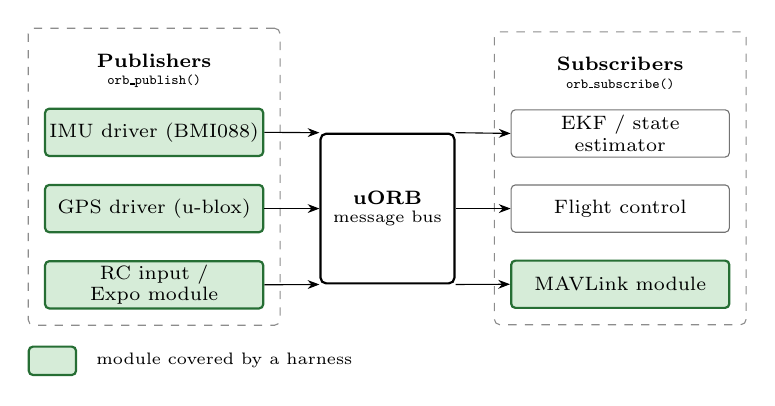
\begin{tikzpicture}[font=\fontsize{7}{8}\selectfont,
 mod/.style={draw,rounded corners=1.5pt,minimum height=6mm,text width=27mm,align=center,inner sep=1pt,fill=white,draw=black!55},
 ver/.style={mod,fill=verfill,draw=verdraw,line width=0.8pt,text=black},
 bus/.style={draw,rounded corners=2pt,minimum height=19mm,minimum width=17mm,align=center,fill=white,thick,inner sep=1pt},
 grp/.style={draw=black!45,dashed,rounded corners=2pt,inner sep=2mm},
 ar/.style={-{Stealth[length=1.5mm]},line width=0.4pt}]
\node[ver] (gps) {GPS driver (u-blox)};
\node[ver,above=3.4mm of gps] (imu) {IMU driver (BMI088)};
\node[ver,below=3.4mm of gps] (rc) {RC input / Expo module};
\node[bus,right=7mm of gps] (uorb) {\textbf{uORB}\\[-1pt]{\fontsize{6}{7}\selectfont message bus}};
\node[mod,right=7mm of uorb] (fc) {Flight control};
\node[mod,above=3.4mm of fc] (ekf) {EKF / state estimator};
\node[ver,below=3.4mm of fc] (mav) {MAVLink module};
\node[above=1.3mm of imu,align=center] (pl) {\textbf{Publishers}\\[-1.5pt]{\fontsize{5.5}{6}\selectfont\texttt{orb\_publish()}}};
\node[above=1.3mm of ekf,align=center] (sl) {\textbf{Subscribers}\\[-1.5pt]{\fontsize{5.5}{6}\selectfont\texttt{orb\_subscribe()}}};
\begin{scope}[on background layer]
\node[grp,fit=(imu)(gps)(rc)(pl)] (gp) {};
\node[grp,fit=(ekf)(fc)(mav)(sl)] (gs) {};
\end{scope}
\draw[ar](imu.east)--(uorb.north west);
\draw[ar](gps.east)--(uorb.west);
\draw[ar](rc.east)--(uorb.south west);
\draw[ar](uorb.north east)--(ekf.west);
\draw[ar](uorb.east)--(fc.west);
\draw[ar](uorb.south east)--(mav.west);
\node[ver,minimum height=3.6mm,minimum width=6mm,text width=0pt,inner sep=0pt,anchor=north west] (lg) at ([yshift=-2.5mm]gp.south west) {};
\node[right=1.2mm of lg,font=\fontsize{6.5}{7.5}\selectfont,anchor=west] {module covered by a harness};
\end{tikzpicture}
}
    \caption{PX4 communication architecture: drivers publish sensor data
    through uORB to estimation, control, and communication
    modules~\cite{PX4_Documentation}. Modules highlighted in green are
    a subset of the twelve modules covered in this work, shown for legibility.}
    \label{fig:px4_arch}
\end{figure}

\section{Related Work}
\label{sec:related}

\paragraph{BMC of firmware and C/C++ code}
BMC tools such as ESBMC and CBMC are commonly evaluated on curated
competition benchmarks~\cite{Beyer2022}.
Sousa et al.~\cite{Sousa2026} applied ESBMC to large open-source C
projects; we inherit their BMC workflow but add two
firmware-specific steps: stub-based hardware I/O abstraction
(\entra{UART, Universal Asynchronous Receiver-Transmitter; I2C,
Inter-Integrated Circuit; SPI, Serial Peripheral Interface;} uORB)
and datasheet-derived custom assertions.

\paragraph{UAV verification and security}
Formal verification of autopilot firmware remains an open
gap~\cite{Luckcuck2019}.
Pollien~\cite{Pollien2023} verified Paparazzi with Frama-C and Coq;
Khatiri et al.~\cite{Khatiri2024}
proposed simulation-based PX4 testing, complementary to BMC.
Bernardeschi et al.~\cite{Bernardeschi2023} applied formal methods at
mission-logic level, not driver code. Unlike
all of these, our target is PX4 Autopilot code at a pinned \texttt{main}-branch commit, analyzed, through harnesses, for bounded absence of memory-safety and overflow
violations rather than tested or monitored at runtime.

\section{Methodology}
\label{sec:methodology}

We propose an eight-stage methodology (Fig.~\ref{fig:methodology}):
(i)~module selection, (ii)~hardware-abstraction stubs,
(iii)~safety-property specification, (iv)~ESBMC execution,
(v)~counterexample analysis, (vi)~community reporting,
(vii)~cross-tool validation and patch verification, and
(viii)~cross-autopilot portability and \entra{continuous
integration/continuous delivery (CI/CD)} integration.
We adopt a modular strategy because PX4's \texttt{src} tree
(${\approx}710$k~LoC) makes monolithic verification impractical.
Stages~(i) and (iv)--(vi) follow the workflow of
Sousa et al.~\cite{Sousa2026}; our additions are the firmware-specific
stages~(ii)--(iii) (hardware-abstraction stubs, datasheet-derived
assertions) and stages~(vii)--(viii), which add cross-tool validation,
patch re-verification, cross-autopilot checking, and CI/CD integration.
\entra{In practice: \corr{stage (v) checks each counterexample against the
unmodified driver source, by replay or by reading the code (Section~\ref{subsec:case-gps}); stage (vi) reports findings to the PX4 community (for GPS and FIFO the upstream issue requested triage and replay came afterwards, Section~\ref{subsec:case-imu})}; stage (vii)
cross-checks with an independent verifier and re-verifies any patch
(\S\ref{subsec:overall}); stage (viii) checks cross-autopilot
reproduction and runs the harnesses in CI on every push
(\S\ref{subsec:discussion}).}

\begin{figure}[t]
\centering
\resizebox{0.9\columnwidth}{!}{%
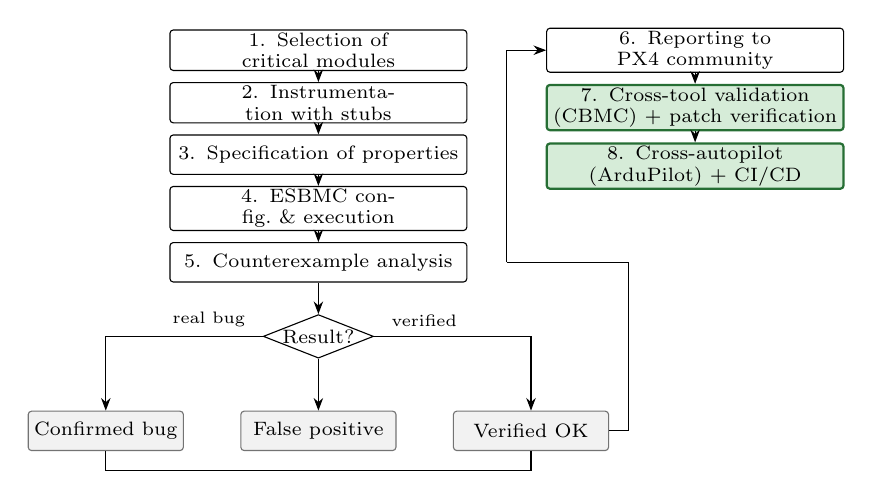
\begin{tikzpicture}[font=\fontsize{7}{8}\selectfont, node distance=1.4mm,
 st/.style={draw,rounded corners=1.2pt,fill=white,minimum height=5mm,text width=37mm,align=center,inner sep=1pt},
 add/.style={st,fill=verfill,draw=verdraw,line width=0.8pt},
 outb/.style={draw,rounded corners=1.2pt,minimum height=5mm,text width=19mm,align=center,inner sep=1pt},
 ar/.style={-{Stealth[length=1.6mm]},line width=0.4pt}]
\node[st] (s1) {1. Selection of critical modules};
\node[st,below=of s1] (s2) {2. Instrumentation with stubs};
\node[st,below=of s2] (s3) {3. Specification of properties};
\node[st,below=of s3] (s4) {4. ESBMC config.\ \& execution};
\node[st,below=of s4] (s5) {5. Counterexample analysis};
\node[st,right=10mm of s1] (s6) {6. Reporting to PX4 community};
\node[add,below=of s6] (s7) {7. Cross-tool validation (CBMC) + patch verification};
\node[add,below=of s7] (s8) {8. Cross-autopilot (ArduPilot) + CI/CD};
\node[diamond,draw,aspect=2.4,inner sep=0pt,minimum width=14mm,below=4mm of s5,fill=white] (d) {Result?};
\node[outb,fill=black!5,draw=black!55] (o1) at ($(d)+(-27mm,-12mm)$) {Confirmed bug};
\node[outb,fill=black!5,draw=black!55] (o2) at ($(d)+(0,-12mm)$) {False positive};
\node[outb,fill=black!5,draw=black!55] (o3) at ($(d)+(27mm,-12mm)$) {Verified OK};
\foreach \a/\b in {s1/s2,s2/s3,s3/s4,s4/s5,s5/d,s6/s7,s7/s8} \draw[ar](\a)--(\b);
\draw[ar](d.west)-|(o1.north); \draw[ar](d.south)--(o2.north); \draw[ar](d.east)-|(o3.north);
\node[font=\fontsize{6}{7}\selectfont,anchor=south east] at ([xshift=-1mm]d.west) {real bug};
\node[font=\fontsize{6}{7}\selectfont,anchor=south west] at ([xshift=1mm]d.east) {verified};
\coordinate (g) at ($(s5.east)+(5mm,0)$);
\draw[line width=0.4pt](o1.south)--++(0,-2.5mm)-|(o3.south);
\draw[line width=0.4pt](o3.east)--++(2.5mm,0)|-(g);
\draw[ar](g)|-(s6.west);
\end{tikzpicture}
}
\caption{Eight-stage verification pipeline. Stages~1 and 4--6 follow
    the workflow of Sousa et al.~\cite{Sousa2026};
    stages~2--3 (hardware stubs, datasheet-derived assertions) and the
    shaded stages~7--8 are the additions of this work.
    None of the three analyzed counterexamples is labeled a
    confirmed bug (Sections~\ref{subsec:case-imu} and~\ref{subsec:case-gps}).}
    \label{fig:methodology}
\end{figure}

As an example, the GPS uBlox driver instantiates every stage: it is
selected by safety impact (i), its I/O is stubbed (ii), the
buffer-bounds property is specified at the \texttt{memcpy} (iii), ESBMC
yields a counterexample
\entra{(iv--v), which is filed
upstream (vi) as Issue~\#26866~\cite{PX4_Issue26866}; the maintainer's review and our source
analysis of the driver's bounds-checking logic then show that the violating
state does not arise in production},
cross-checked with CBMC and re-verified on the patch (vii), and
recorded for CI (viii); Section~\ref{subsec:case-gps} details this
trace and its violation.
\subsection{Module Selection and Harness Construction}
\label{subsec:harnesses}
Modules are prioritized by safety impact on the sensing-to-actuation
path and feasibility of stub-based isolation; selecting by stub
feasibility introduces a selection bias (Section~\ref{sec:threats}).
We wrote harnesses for twelve modules by hand, totaling
${\approx}2{,}800$ lines, summarized
per module in Table~\ref{tab:benchmarks}.

\begin{table}[t]
\centering
\caption{Modules covered: target size, harness size, PX4 source
location, and selection rationale (input class exercised).}
\label{tab:benchmarks}
\scriptsize
\setlength{\tabcolsep}{3pt}
\begin{tabular}{@{}llrrl@{}}
\toprule
\textbf{Module} & \textbf{PX4 path (\texttt{src/})} & \textbf{Tgt.} & \textbf{Harn.} & \textbf{Input class}\\
\midrule
GPS uBlox      & \texttt{drivers/gps}          & 1712 & 294 & Serial sensor \\
IMU BMI088     & \texttt{drivers/imu/.../bmi088} & 700 & 319 & Serial sensor \\
MAVLink        & \texttt{modules/mavlink}       & 3624 & 82 & Telemetry link \\
Expo RC        & \texttt{lib/mathlib/math}      & 303 & 129 & Radio input \\
Battery Mon.   & \texttt{lib/battery}           & 449 & 242 & Power sensor \\
PWM Output        & \texttt{drivers/pwm\_out}      & 337 & 208 & Actuation \\
RC Update      & \texttt{modules/rc\_update}     & 769 & 253 & Radio input \\
Navigator      & \texttt{modules/navigator}     & 497 & 291 & Mission logic \\
EKF2 Cov.      & \texttt{modules/ekf2/EKF}      & 385 & 296 & State estim. \\
Magnetometer   & \texttt{modules/sensors}       & 792 & 239 & Serial sensor \\
Barometer      & \texttt{lib/sensor\_calibration} & 246 & 278 & Serial sensor \\
VTOL           & \texttt{modules/vtol\_att\_control} & 591 & 146 & Actuation \\
\bottomrule
\multicolumn{5}{l}{Tgt.=LoC of the PX4 source file(s) the harness excerpts (pinned commit);}\\
\multicolumn{5}{l}{Harn.=harness LoC (both \texttt{wc\,-l});}\\
\multicolumn{5}{l}{\entra{RC=radio control; IMU=Inertial Measurement Unit;}}\\
\multicolumn{5}{l}{\entra{EKF2=Extended Kalman Filter 2; PWM=Pulse-Width Modulation.}}\\
\multicolumn{5}{l}{Modules selected by safety impact and stub feasibility.}
\end{tabular}
\end{table}
\entra{Instrumenting a module requires three artifacts written by hand:
an entry-point harness driving the module with non-deterministic inputs,
stubs replacing hardware and middleware I/O (UART, I2C, SPI, uORB), and
the datasheet-derived assertions.} \entra{All three live in the same
\texttt{test\_*.cpp} file per module; the repository has no separate
stub files.} \entra{Against ${\approx}10{,}400$ lines of
target code, this is a ratio near $1{:}3.7$, with per-module figures in
Table~\ref{tab:benchmarks}. PX4 sources were not modified.}

Rather than a line-coverage percentage, which would mislead when each
harness stubs most of its module and explores only paths reachable
under $k=10$, we characterize coverage by \emph{input category}
(Section~\ref{subsec:overall}). Hardware I/O, NuttX calls, and inter-module dependencies are
replaced by stubs returning \texttt{nondet\_T()} values.
Each harness provides an entry point with stubs and assertions.
\entra{The GPS uBlox harness, for instance, is one of five test functions
in its file (\texttt{test\_choice=3} in \texttt{main}) and is the function
that produces the counterexample analyzed in
Section~\ref{subsec:case-gps}: it draws a non-deterministic
\texttt{input\_len} and \texttt{dump\_buffer.len}, constrains them via
\texttt{\_\_ESBMC\_assume} to
\texttt{input\_len}$\,\in\,(0,\text{GPS\_DUMP\_DATA\_SIZE}{+}10]$ and
\texttt{dump\_buffer.len}$\,\geq\,\text{GPS\_DUMP\_DATA\_SIZE}{-}5$, calls
\texttt{dumpGpsData()}, and asserts the resulting buffer length stays
within \texttt{GPS\_DUMP\_DATA\_SIZE} \corr{(this final assertion is a tautology, as its last disjunct $(\texttt{len}\,\&\,\texttt{0x7F})\le 200$ always holds, so the violation is caught by ESBMC's automatic dereference check inside \texttt{memcpy})}. These bounds admit the
values in the counterexample (\texttt{input\_len=10}, \texttt{dump\_buffer.len=207}),
which lead to the out-of-bounds \texttt{memcpy} shown in
Listing~\ref{lst:bug-gps}.}
Harness sources are in the artifact repository~\cite{Artifact2026}\entra{, which contains the twelve test
harnesses (one \texttt{test\_*.cpp} file per module), raw ESBMC logs for every run reported here, CBMC
cross-validation scripts and logs, per-module command lines, and a
reproduction guide; it does not yet contain separate replay-driver
files or sanitizer logs (replay is described in prose,
Section~\ref{subsec:case-gps}).}

\subsection{Safety Properties}
\label{subsec:properties}

\emph{Automatic} properties (array bounds, pointer safety,
arithmetic overflow, division by zero~\cite{Menezes2024,Monteiro2022}) are enabled uniformly.
\emph{Custom} properties encode datasheet requirements.
The BMI088 datasheet~\cite{Bosch2022} restricts operating temperature
to $[-40,\,+85]\,^\circ$C. Because the driver's affine conversion is unclamped, any raw reading outside this range violates
$\phi_{\text{temp}}$ by construction; we therefore treat
$\phi_{\text{temp}}$ not as a hardware guarantee but as a
\emph{coverage probe} that flags \emph{missing input-range validation}
in the driver:
\begin{equation}
  \phi_{\text{temp}}: \quad -40.0 \leq \textit{temperature} \leq 85.0
  \label{eq:prop_temp}
\end{equation}
\entra{The GPS driver requires the dump buffer fill level to stay within
the record capacity, \texttt{sizeof(dump\_data->data)}; the harness models
it with the macro \texttt{GPS\_DUMP\_DATA\_SIZE}:}
\begin{equation}
  \phi_{\text{gps}}: \quad \textit{dump\_data.len} \leq \texttt{GPS\_DUMP\_DATA\_SIZE}
  \label{eq:prop_gps}
\end{equation}
Since \texttt{len} is a free input, checking $\phi_{\text{gps}}$ at
entry would be trivially violated by the input itself; we check the access at the \texttt{memcpy} use site,
where the driver must not access past the buffer for any \texttt{len}.
Counterexamples are checked against the unmodified source to rule out stub artifacts (by replay or by reading the code); replay drivers are not yet in the artifact.

\section{Experimental Evaluation}
\label{sec:results}

This section evaluates the methodology on harnesses of twelve
PX4 modules. We address three research questions: \textbf{RQ1}:
What is the per-module verification latency on commodity
hardware? \textbf{RQ2}: Does BMC expose model-reachable violations
that existing PX4 unit tests do not exercise? \textbf{RQ3}: Which
per-module configurations are needed to make each module
tractable?

\subsection{Experimental Setup}
\label{subsec:setup}

Verification ran on an Intel~i7-13700K / 64~GB / Ubuntu~24.04
against PX4 \texttt{main}-branch sources (commit~\texttt{8be2590c15},
2026-06-04); the complete artifact (harnesses and logs) is
archived on Zenodo, DOI~\texttt{10.5281/zenodo.23282236}~\cite{Zenodo2026}.
Reported times are the median of three runs. The commit is
2{,}935 commits after v1.16.0 and after the v1.17.0 release;
the harnesses are copies of source excerpts, not compiled
against PX4 files, and some constants differ (GPS buffer: 200
bytes in the harness, 79 in PX4), so the VCCs cover the
harnesses, not the full modules. All harnesses were verified
with ESBMC~v8.1.0 using Boolector~3.2.4~\cite{Brummayer2009} as the
solver.\footnote{The version string \texttt{ESBMC version 8.1.0} was read
from all twelve run logs; the BMI088 and GPS counterexamples were
originally filed upstream (Issues~\#26865~\cite{PX4_Issue26865},
\#26866~\cite{PX4_Issue26866}) from earlier runs (ESBMC~v7.10;
GPS 12.1\,s), with times and counterexample values here taken from the
v8.1.0 logs.}
Boolector is also the configuration under which the upstream
GPS report (Issue~\#26866~\cite{PX4_Issue26866}) was filed; in earlier exploratory
runs Z3 returned no verdict on the GPS harness
(Section~\ref{sec:threats}). \
\noindent\begin{minipage}{\columnwidth}
Default invocation:
\begin{lstlisting}[language=bash,breaklines=true]
esbmc module.cpp --unwind 10 --no-unwinding-assertions \
  --overflow-check --default-solver boolector \
  --timeout 120s
\end{lstlisting}
\end{minipage}
Since \texttt{--no-unwinding-assertions} is set, loops exceeding
$k=10$ are silently truncated (Section~\ref{sec:threats}).
Adjustments: MAVLink used \texttt{--unwind~300}; Navigator/Mission
\texttt{--unwind~15}; VTOL \texttt{--no-library}, which disables
ESBMC's abstract C library: \texttt{sinf}/\texttt{sqrtf} then return
nondeterministic values, an over-approximation under which no
violation of the remaining checks is missed; the
library-internal checks, however, are no longer verified, so the verdict covers correspondingly fewer properties.
\subsection{Overall Results}
\label{subsec:overall}

Table~\ref{tab:results} summarizes outcomes. Harnesses for ten of twelve modules
verify with no violation up to the bound; this
bounded, model-level evidence is the campaign's primary outcome
(scope qualified in Section~\ref{sec:threats}).
The GPS~uBlox harness yielded the one violation
(Issue~\#26866~\cite{PX4_Issue26866}); the BMI088 FIFO-counter candidate
was a false positive on triage; the
temperature-range observation remains contested
(Section~\ref{subsec:case-imu}).
\begin{table}[t]
\centering
\caption{Verification results for harnesses of twelve PX4 modules.}
\label{tab:results}
\scriptsize
\setlength{\tabcolsep}{3pt}
\begin{tabular}{@{}lcrccr@{}}
\toprule
\textbf{Module} & \textbf{Outcome} & \textbf{MRV}$^\P$ & \textbf{Unw.} & \textbf{Solver} & \textbf{Time}$^\|$\\
\midrule
IMU BMI088        & \textit{viol.} & 0$^\ddagger$ & 10 & Bool.$^\star$ & 0.1\,s$^{\#}$ \\
GPS uBlox         & \textit{viol.} & 1 & 10 & Bool.$^\star$ & 64.9\,s \\
MAVLink Parser    & \textit{no viol.} & 0 & 300 & Bool. & 49.2\,s \\
Expo RC           & \textit{no viol.} & 0 & 10 & Bool. & 4.9\,s \\
Battery Monitor   & \textit{no viol.} & 0 & 10 & Bool. &   6.7\,s \\
PWM Output        & \textit{no viol.} & 0 & 10 & Bool. &   0.2\,s \\
RC Update         & \textit{no viol.} & 0 & 10 & Bool. &  9.5\,s \\
Navigator/Mission & \textit{no viol.} & 0 & 15 & Bool. &   0.1\,s \\
EKF2 Covariance   & \textit{no viol.} & 0 & 10 & Bool. & 12.2\,s \\
Magnetometer      & \textit{no viol.} & 0 & 10 & Bool. &  6.6\,s \\
Barometer         & \textit{no viol.} & 0 & 10 & Bool. &   0.4\,s \\
VTOL$^\S$         & \textit{no viol.} & 0 & 10 & Bool. &  4.0\,s \\
\midrule
\textbf{Total} & \textit{10 no viol., 2 viol.} & 1 & --- & --- & ${\approx}94$\,s$^{\S\S}$ \\
\bottomrule
\multicolumn{6}{l}{\textit{no viol.}$=$no violation up to $k$; \textit{viol.}$=$violation found.}\\
\multicolumn{6}{l}{$^\P$MRV=model-reachable violations (not confirmed defects).}\\
\multicolumn{6}{l}{$^\star$ESBMC v8.1.0; Boolector~3.2.4 for all modules.}\\
\multicolumn{6}{l}{$^\ddagger$FIFO false positive; temperature declined upstream.}\\
\multicolumn{6}{l}{\corr{$^{\S\S}$93.8\,s for the ten completed modules; 158.7\,s with GPS (64.9\,s).}}\\
\multicolumn{6}{l}{$^\S$VTOL \texttt{--no-library}: library-internal checks not verified.}\\
\multicolumn{6}{l}{$^\|$Median of three runs.}\\
\multicolumn{6}{l}{$^{\#}$Violating modules stop at the first violation (decision time).}
\end{tabular}
\end{table}
Times ranged $0.1$--$64.9$\,s; CI wall-clock times were
not measured (Section~\ref{subsec:discussion}).
\begin{rqbox}
\textbf{These results answer RQ1}: every timed harness verifies in under
ninety seconds on commodity hardware. Since each is checked in isolation
through a small harness, this demonstrates per-module
\emph{feasibility}, not whole-system scaling.
\end{rqbox}

The modules covered are not a uniform sample: they sit on the
safety-critical sensing-to-actuation path, covering the
representative untrusted-input classes, namely serial sensor buses, the
radio/telemetry link, actuation, estimation, and mission logic
(Table~\ref{tab:benchmarks}).
The remainder is dominated by ground-station, logging, and
build code with low runtime-safety consequence; the flight-critical
exceptions (commander, failsafe, geofence) are priority future work
(Section~\ref{sec:conclusion}; remaining gaps in
Section~\ref{sec:threats}).

To assess tool-specificity, we ran CBMC~5.95.1~\cite{Kroening2014}
with matching options (\texttt{--unwind~10},
overflow and bounds checks, no unwinding assertions) and the same
$120$\,s timeout, on a separate, reduced harness for IMU~BMI088 (both tools agreed) and on a separate harness for GPS~uBlox. For GPS~uBlox,
under \corr{the later CBMC harness (added 2026-09-24; the original, with \texttt{len}~$<$~$200$, returned \textsc{verification successful} in Issue~\#26866~\cite{PX4_Issue26866}, as its precondition excludes the violating states) with the} precondition \texttt{len}~$\geq$~$190$
(\texttt{GPS\_DUMP\_DATA\_SIZE}$\,-\,$10, seeding the length field near
the buffer boundary\corr{; the ESBMC harness uses $-5$}), both tools flag a violation, but CBMC only at reduced bounds (\texttt{--unwind~2}, \texttt{3} and~\texttt{5}: unwritable \texttt{memcpy} destination); at \texttt{--unwind~10} it did not finish within a longer $30$\,min limit.
ESBMC reports an out-of-bounds access inside \texttt{memcpy}
(a dereference failure); we label the underlying defect CWE-191 (the unsigned
underflow) leading to CWE-119/787 (the out-of-bounds write), a classification
of ours rather than a tool output \entra{(not a confirmed defect,
Section~\ref{subsec:case-gps}).}
Agreement under the same precondition corroborates only the encoding, not
that the state arises in the production driver
(Section~\ref{subsec:case-gps}).

\subsection{Case Study: IMU BMI088 Driver}
\label{subsec:case-imu}

The BMI088 driver (700~LoC) produced
two candidates; the analysis led to different conclusions for each.

\subsubsection{Temperature out of operating range (contested, rejected upstream)}
The driver does not validate temperature before thermal-compensation
arithmetic; the BMI088 datasheet~\cite{Bosch2022} restricts operation
to $[-40,\,+85]\,^\circ$C (Eq.~\eqref{eq:prop_temp}).
ESBMC produced \texttt{temp\_msb=63}, \texttt{temp\_lsb=95}
(\texttt{Temp\_uint11=506}), yielding $86.25\,^\circ$C
(Listing~\ref{lst:bug-temp}).
This is CWE-1284 (improper validation of quantity): the driver consumes a
reading outside the certified range unchecked.
\entra{The harness needs no \texttt{\_\_ESBMC\_assume} here: its two fully
non-deterministic 8-bit inputs already span the sensor's 11-bit raw-value
range, so the assertion is exercised over the reachable register domain
rather than vacuously.}
Whether this is a defect is contested. \corr{In review of the upstream patch (PX4~PR~\#27575~\cite{PX4_PR27575}), a reviewer objected to clamping the value (``faking the number'') and asked what the sensor itself reports outside its operating range; a maintainer then closed the PR because it does not follow the pattern established in other drivers. Issue~\#26865~\cite{PX4_Issue26865} was closed automatically as not planned.}
We
retain the observation only as a design note with \emph{no confirmed
safety consequence and no accepted remediation}, illustrating the
triage step of the methodology rather than a defect.

\begin{lstlisting}[float=t,basicstyle=\ttfamily\scriptsize,
numbers=none,language={},captionpos=b,
caption={ESBMC counterexample: BMI088 temperature $86.25\,^\circ$C
$>$ $85\,^\circ$C. Missing input-range validation (CWE-1284).},
label=lst:bug-temp]
[Counterexample]
State 2 -- test_temperature_calculation, line 120
  temp_msb = 63, temp_lsb = 95
State 7 -- updateTemperature, line 42
  Temp_uint11 = 506
State 11 -- updateTemperature, line 51
  temperature = 86.250000f
Violated property: assertion
  temperature >= -40.0f && temperature <= 85.0f

VERIFICATION FAILED
\end{lstlisting}

\subsubsection{FIFO counter candidate (false positive)}
ESBMC produced \texttt{count=9088}~bytes (over $8\times$ the
$1{,}024$-byte FIFO), suggesting CWE-190/CWE-787.
Checking this counterexample against the
\emph{uninstrumented} production driver showed a \textbf{false
positive}. The released driver guards the read on three levels:
\begin{itemize}
  \item the byte counter is compared against the FIFO size and reset
        whenever \texttt{fifo\_byte\_counter}~$\geq$~\texttt{FIFO::SIZE};
  \item the sample count is bounded to \texttt{FIFO\_MAX\_SAMPLES};
  \item and transfer length is clamped via\\
        \texttt{math::min(samples*sizeof(FIFO::DATA)+4, FIFO::SIZE)}.
\end{itemize}
The value $9088\geq1{,}024$ triggers the first guard reset,
so no out-of-bounds access is reachable. The candidate arose
because the harness omitted these guards. A clamp for it was also
proposed upstream in the same PR~\#27575~\cite{PX4_PR27575}, but inspection of
the production driver shows the candidate is a false positive. The
check against the production source caught it.

\subsection{Case Study: GPS uBlox Driver}
\label{subsec:case-gps}

The uBlox harness (excerpting a $1{,}712$~LoC source file) was checked in $64.9$\,s.
The available-space check subtracts the buffer fill level from the capacity (the harness defines \texttt{GPS\_DUMP\_DATA\_SIZE} as $200$; the released driver declares \texttt{uint8[79]~data}):
\begin{lstlisting}[language=C]
if (write_len > GPS_DUMP_DATA_SIZE - dump_data->len)
\end{lstlisting}
When \texttt{dump\_data->len} exceeds the capacity, the difference is negative ($-7$ for $\texttt{len}=207$: the \texttt{uint8\_t} length is promoted to \texttt{int}, so the subtraction is signed in the harness) and converts to an enormous \texttt{size\_t} value at the comparison with \texttt{write\_len}, rendering the guard always false.
ESBMC produced \texttt{input\_len=10} and
\texttt{dump\_data->len=207}; the guard is then always false and the
subsequent \texttt{memcpy} writes outside the buffer (Listing~\ref{lst:bug-gps}).
CWE-191 (Integer Underflow) $\to$ CWE-119
(Memory Buffer Bounds Violation).
On MMU-less Pixhawk hardware an out-of-bounds write could corrupt
adjacent memory; under NuttX's flat memory model it need not raise a
clean fault\entra{, though reachability on the production driver,
established next, bounds the physical
impact.}

\entra{\corr{As the PX4 maintainer (mrpollo) showed in the review of PR~\#27576~\cite{PX4_PR27576}, and as source analysis then confirmed,} the production driver resolves this question
negatively: the write loop clamps \texttt{write\_len} to the remaining
free space, so the fill level never exceeds the buffer before the record
is published and the field reset to zero. The violation is thus
reachable in the model but not in the production driver. We retain it as
an example of why a formally valid counterexample must be checked against production code before it is called a defect.}
\begin{rqbox}
\textbf{These results answer RQ2} in the affirmative for at least one
module: BMC exposed a model-reachable memory-safety violation in the
GPS driver harness that the existing PX4 unit tests do not exercise.
\end{rqbox}

\begin{lstlisting}[float=t,basicstyle=\ttfamily\scriptsize,
numbers=none,language={},captionpos=b,
caption={ESBMC counterexample: unsigned underflow in
\texttt{dumpGpsData()} propagates to out-of-bounds \texttt{memcpy}
(CWE-191 $\rightarrow$ CWE-119). The harness's local
\texttt{dump\_buffer} is the \texttt{dump\_data} buffer passed to
the driver.},label=lst:bug-gps]
[Counterexample]
State 3 -- test_gps_real_bit_operation, line 179
  input_len = 10
State 8 -- test_gps_real_bit_operation, line 185
  dump_buffer.len = 207
State 21 -- __memcpy_impl, line 280
  Violated property: dereference failure:
  Access to object out of bounds

VERIFICATION FAILED
\end{lstlisting}

\paragraph{Patch verification}
On the patched harness, CBMC~5.95.1 reports $0/7$ failed properties (PR~\#27576~\cite{PX4_PR27576}; log in the artifact). This is a check of the proposed guard on the harness, not evidence about the production driver: the unpatched CBMC harness reports the same $0/7$ under the same bounded-length precondition, so the comparison does not isolate the guard's effect. ESBMC fails on the unpatched harness (Table~\ref{tab:results}); the artifact has no ESBMC log for the patched harness.

\subsection{Discussion}
\label{subsec:discussion}

\paragraph{Configuration, soundness, and time}
\begin{rqbox}
\textbf{These results answer RQ3}: three per-module configurations
suffice; MAVLink \texttt{--unwind~300} (deep parsing loops), VTOL
\texttt{--no-library} (disables the abstract C library),
and Navigator \texttt{--unwind~15} are all documented in the artifact
repository.
\end{rqbox}
A \texttt{grep} over the PX4 test tree finds no unit test referencing
\texttt{dumpGpsData} or the \texttt{GPS} class (absence of
\emph{direct} coverage only; \entra{software-in-the-loop (SITL)} tests may still exercise it), so BMC and unit testing remain
complementary~\cite{Godefroid2005,Khatiri2024}.

\paragraph{Cross-autopilot observation and CI/CD}
The same missing-range-validation observation (CWE-1284) appears in
ArduPilot's equivalent driver~\cite{ArduPilot}: running CBMC~5.95.1 against
\texttt{AP\_InertialSensor\_BMI088.cpp} (lines~383--385) reproduces it (ArduPilot
Issue~\#33272~\cite{ArduPilot_Issue33272}).
\corr{An ArduPilot maintainer closed the issue, citing the datasheet's $-104$ to $150\,^\circ$C measurement range.} Both projects declined it; we report it only
as a consistency check.
A GitHub Actions workflow in a PX4
fork~\cite{PX4_Fork}
runs the IMU and GPS harnesses on every push and pull request.

\section{Threats to Validity}
\label{sec:threats}

\paragraph{Internal validity}
Reported times (medians of three runs) are orders-of-magnitude only.
Triage discarded two further early candidates (MAVLink, EKF2) as configuration artifacts; their logs are not in the artifact. The GPS underflow was found with Boolector; Z3 returned no verdict within the timeout (as did MAVLink and EKF2 at \texttt{--unwind~10} in our 8.1 re-runs), so the result depends on the solver;
the CBMC cross-check is partial for GPS (reduced bound).

\paragraph{External validity}
Selecting modules by stub feasibility under-represents modules with
heavy hardware or scheduler coupling, so the sample is not
statistically representative of PX4. Modular analysis misses
integration bugs from concurrent interactions.

\paragraph{Construct validity}
Verification was bounded at $k=10$, and with
\texttt{--no-unwinding-assertions} enabled, loops that exceed the
bound are silently truncated, so a \textsc{successful} verdict can
hide false negatives even below the intended operational
depth.

\paragraph{Stub soundness}
Stubs returning \texttt{nondet\_T()} over-approximate hardware
\emph{inputs}, so a harness that omits production guards can admit
states the real driver rejects, as the FIFO candidate showed;
genuineness rests on checking against the production source. Conversely, stubs
\emph{under-approximate} internal hardware behavior (I2C/SPI state
machines, NuttX scheduling), so defects triggered by such internal
state would go undetected.

\section{Conclusion and Future Work}
\label{sec:conclusion}

We presented a systematic verification methodology over harnesses of twelve PX4
Autopilot modules (commit \texttt{8be2590c15}); its primary outcome is bounded, model-level
assurance, with harnesses for ten modules, spanning representative untrusted-input
classes, verified free of memory-safety and overflow violations up to
the bound (${\approx}94$\,s in total; ${\approx}159$\,s with GPS). ESBMC also surfaced a
memory-safety violation in the GPS uBlox driver harness
\entra{(Issue~\#26866~\cite{PX4_Issue26866}), \corr{reproduced with CBMC under a seeded harness at a reduced bound} and proposed upstream
with a guard (PR~\#27576~\cite{PX4_PR27576}); the PX4 maintainer's review, confirmed by source analysis of the production
driver, subsequently placed the violating state out of reach there and framed the guard as defensive hardening.}
\entra{The} BMI088 FIFO candidate was a false positive on
source inspection, and the temperature observation was declined.
Future work: k-induction, commander, failsafe and geofence modules,
and PX4 CI with Hardware-in-the-Loop (HIL) evaluation.

\section*{Acknowledgment}
M.A.R. thanks Prof. Lucas C. Cordeiro and Prof. Jos\'e Reginaldo H. de Carvalho for their supervision. The authors thank the SAGRES project and the PX4 development community. This work was carried out at the Federal University of Amazonas (UFAM), with scholarship support from CAPES\corr{ (Finance Code 001)}. Generative AI (Claude, Anthropic) was used for code analysis and for drafting and revising the text; the authors reviewed and take responsibility for all content.

\bibliographystyle{IEEEtran}
{\scriptsize\bibliography{references}}




\end{document}
